\section*{Modulebeschrijving}
\begin{tabularx}{\textwidth}{|>{\columncolor{lichtGrijs}} p{.26\textwidth}|X|}
	\hline
	\textbf{Module name:} & \modulenaam\\
	\hline
	\textbf{Module code: }& \modulecode\\
	\hline
	\textbf{Studie points \newline and hours of effort:} & This module gives \stdPunten studie points, in correspondance with \red{???} hours:
	\begin{itemize}
		\item \red{???} minutes frontal lecture
		\item \red{???} minutes practicum
		\item \red{???} minutes self-study
		\item \red{???} minutes project work
	\end{itemize} \\
	\hline
	\textbf{Examination:} & Projects and tests (open questions and multiple choice) \\
	\hline
	\textbf{Course structure:} & Lectures, self-study, and projects \\
	\hline
	\textbf{Prerequisite knowledge:}& All first and second year programming courses, and all courses in functional programming. \\
	\hline
	\textbf{Learning tools:}  &
		For the security part:
		\begin{itemize}
			\item Book: Everyday Cryptography ISBN-13: 978-0199695591
			\item Book: Cryptography Engineering ISBN-13: 978-0470474242
			\item Book: Threat Modeling Book
			\item PDF: Security Engineering
			\item Usable Security: History, Themes, and Challenges
			\item Book: The art of software security assessment ISBN-13: 978-0321444424
			\item Book: Phishing Dark Waters: The Offensive and Defensive Sides of Malicious Emails ISBN: 978-1-118-95847-6
		\end{itemize} \\
	
		For the formal methods part:
		\begin{itemize}
			\item Book: Friendly F\# (Fun with game programming Book 1), authors: Giuseppe Maggiore, Giulia Costantini
			\item Reader: Friendly F\# (Fun with logic programming), authors: Giuseppe Maggiore, Giulia Costantini, Francesco Di Giacomo, Gerard van Kruining
		\end{itemize} \\
	\hline
	\textbf{Connected to \newline competences:} &
	\begin{center}
		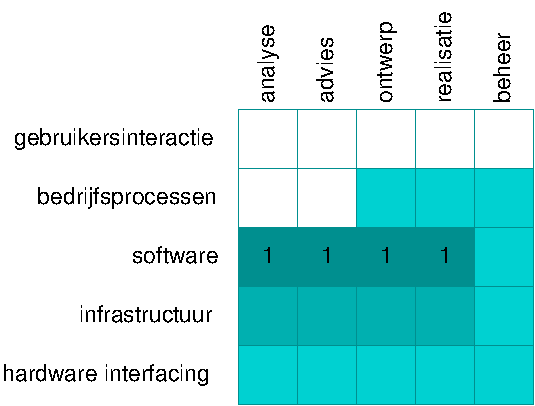
\includegraphics[width=7cm]{img/comptabel.pdf}
	\end{center}\\
	\hline
	\textbf{Learning objectives:}&
	In the context of security, the student can:
	\begin{itemize}
		\item formulate strategies to adequately evaluate security
		\item dissect and construct the layers and objects of security
		\item apply and engage in the red vs blue team method either in the context of implementing/configuring or in the context of sketching/architecting
		\item apply and engage in the white box / laboratory study method either in the context of a code review or in the context of a user study
		\item apply and engage in the black box/field study method either in the context of a \textit{pentest} or in the context of a phishing campaign
	\end{itemize} \\

	In the context of formal methods, the student can:
	\begin{itemize}
		\item abstract complex properties
		\item encode these complex properties into languages, tools, and other libraries
		\item dissect the layers and objects of languages, tools, and other libraries
		\item architect languages, tools, and other libraries in a formal specification
		\item build languages, tools, and other libraries within a functional, logic, or declarative programming language
	\end{itemize} \\
	\hline
\end{tabularx}
\newpage

\begin{tabularx}{\textwidth}{|>{\columncolor{lichtGrijs}} p{.26\textwidth}|X|}
	\hline
	\textbf{Content:}&
	For the security part:
	\begin{itemize}
		\item \red{...}
	\end{itemize}\\
	
	For the formal methods part:
	\begin{itemize}
		\item Functional programming, with special focus on F\#
		\item Meta-programming within F\#
		\item Meta-compilers, with special focus on the school's own implementation
	\end{itemize}\\
	\hline
	\textbf{Modulebeheerders:} & \author\\
	\hline
	\textbf{Date:} & \today \\
	\hline
\end{tabularx}
\newpage
